\documentclass[10pt,a4paper,onecolumn]{article}
\usepackage{marginnote}
\usepackage{graphicx}
\usepackage{xcolor}
\usepackage{authblk,etoolbox}
\usepackage{titlesec}
\usepackage{calc}
\usepackage{tikz}
\usepackage{hyperref}
\hypersetup{colorlinks,breaklinks,
            urlcolor=[rgb]{0.0, 0.5, 1.0},
            linkcolor=[rgb]{0.0, 0.5, 1.0}}
\usepackage{caption}
\usepackage{tcolorbox}
\usepackage{amssymb,amsmath}
\usepackage{ifxetex,ifluatex}
\usepackage{seqsplit}
\usepackage{fixltx2e} % provides \textsubscript
\usepackage[
  backend=biber,
%  style=alphabetic,
%  citestyle=numeric
]{biblatex}
\bibliography{paper.bib}


% --- Page layout -------------------------------------------------------------
\usepackage[top=3.5cm, bottom=3cm, right=1.5cm, left=1.0cm,
            headheight=2.2cm, reversemp, includemp, marginparwidth=4.5cm]{geometry}

% --- Default font ------------------------------------------------------------
% \renewcommand\familydefault{\sfdefault}

% --- Style -------------------------------------------------------------------
\renewcommand{\bibfont}{\small \sffamily}
\renewcommand{\captionfont}{\small\sffamily}
\renewcommand{\captionlabelfont}{\bfseries}

% --- Section/SubSection/SubSubSection ----------------------------------------
\titleformat{\section}
  {\normalfont\sffamily\Large\bfseries}
  {}{0pt}{}
\titleformat{\subsection}
  {\normalfont\sffamily\large\bfseries}
  {}{0pt}{}
\titleformat{\subsubsection}
  {\normalfont\sffamily\bfseries}
  {}{0pt}{}
\titleformat*{\paragraph}
  {\sffamily\normalsize}


% --- Header / Footer ---------------------------------------------------------
\usepackage{fancyhdr}
\pagestyle{fancy}
\fancyhf{}
%\renewcommand{\headrulewidth}{0.50pt}
\renewcommand{\headrulewidth}{0pt}
\fancyhead[L]{\hspace{-0.75cm}\includegraphics[width=5.5cm]{joss-logo.png}}
\fancyhead[C]{}
\fancyhead[R]{}
\renewcommand{\footrulewidth}{0.25pt}

\fancyfoot[L]{\footnotesize{\sffamily Pitkin, (2018). psrqpy: a python interface for querying the ATNF pulsar catalogue. \textit{Journal of Open Source Software}, 3(22), 538. \href{https://doi.org/10.21105/joss.00538}{https://doi.org/10.21105/joss.00538}}}


\fancyfoot[R]{\sffamily \thepage}
\makeatletter
\let\ps@plain\ps@fancy
\fancyheadoffset[L]{4.5cm}
\fancyfootoffset[L]{4.5cm}

% --- Macros ---------

\definecolor{linky}{rgb}{0.0, 0.5, 1.0}

\newtcolorbox{repobox}
   {colback=red, colframe=red!75!black,
     boxrule=0.5pt, arc=2pt, left=6pt, right=6pt, top=3pt, bottom=3pt}

\newcommand{\ExternalLink}{%
   \tikz[x=1.2ex, y=1.2ex, baseline=-0.05ex]{%
       \begin{scope}[x=1ex, y=1ex]
           \clip (-0.1,-0.1)
               --++ (-0, 1.2)
               --++ (0.6, 0)
               --++ (0, -0.6)
               --++ (0.6, 0)
               --++ (0, -1);
           \path[draw,
               line width = 0.5,
               rounded corners=0.5]
               (0,0) rectangle (1,1);
       \end{scope}
       \path[draw, line width = 0.5] (0.5, 0.5)
           -- (1, 1);
       \path[draw, line width = 0.5] (0.6, 1)
           -- (1, 1) -- (1, 0.6);
       }
   }

% --- Title / Authors ---------------------------------------------------------
% patch \maketitle so that it doesn't center
\patchcmd{\@maketitle}{center}{flushleft}{}{}
\patchcmd{\@maketitle}{center}{flushleft}{}{}
% patch \maketitle so that the font size for the title is normal
\patchcmd{\@maketitle}{\LARGE}{\LARGE\sffamily}{}{}
% patch the patch by authblk so that the author block is flush left
\def\maketitle{{%
  \renewenvironment{tabular}[2][]
    {\begin{flushleft}}
    {\end{flushleft}}
  \AB@maketitle}}
\makeatletter
\renewcommand\AB@affilsepx{ \protect\Affilfont}
%\renewcommand\AB@affilnote[1]{{\bfseries #1}\hspace{2pt}}
\renewcommand\AB@affilnote[1]{{\bfseries #1}\hspace{3pt}}
\makeatother
\renewcommand\Authfont{\sffamily\bfseries}
\renewcommand\Affilfont{\sffamily\small\mdseries}
\setlength{\affilsep}{1em}


\ifnum 0\ifxetex 1\fi\ifluatex 1\fi=0 % if pdftex
  \usepackage[T1]{fontenc}
  \usepackage[utf8]{inputenc}

\else % if luatex or xelatex
  \ifxetex
    \usepackage{mathspec}
  \else
    \usepackage{fontspec}
  \fi
  \defaultfontfeatures{Ligatures=TeX,Scale=MatchLowercase}

\fi
% use upquote if available, for straight quotes in verbatim environments
\IfFileExists{upquote.sty}{\usepackage{upquote}}{}
% use microtype if available
\IfFileExists{microtype.sty}{%
\usepackage{microtype}
\UseMicrotypeSet[protrusion]{basicmath} % disable protrusion for tt fonts
}{}

\usepackage{hyperref}
\hypersetup{unicode=true,
            pdftitle={psrqpy: a python interface for querying the ATNF pulsar catalogue},
            pdfborder={0 0 0},
            breaklinks=true}
\urlstyle{same}  % don't use monospace font for urls
\usepackage{graphicx,grffile}
\makeatletter
\def\maxwidth{\ifdim\Gin@nat@width>\linewidth\linewidth\else\Gin@nat@width\fi}
\def\maxheight{\ifdim\Gin@nat@height>\textheight\textheight\else\Gin@nat@height\fi}
\makeatother
% Scale images if necessary, so that they will not overflow the page
% margins by default, and it is still possible to overwrite the defaults
% using explicit options in \includegraphics[width, height, ...]{}
\setkeys{Gin}{width=\maxwidth,height=\maxheight,keepaspectratio}
\IfFileExists{parskip.sty}{%
\usepackage{parskip}
}{% else
\setlength{\parindent}{0pt}
\setlength{\parskip}{6pt plus 2pt minus 1pt}
}
\setlength{\emergencystretch}{3em}  % prevent overfull lines
\providecommand{\tightlist}{%
  \setlength{\itemsep}{0pt}\setlength{\parskip}{0pt}}
\setcounter{secnumdepth}{0}
% Redefines (sub)paragraphs to behave more like sections
\ifx\paragraph\undefined\else
\let\oldparagraph\paragraph
\renewcommand{\paragraph}[1]{\oldparagraph{#1}\mbox{}}
\fi
\ifx\subparagraph\undefined\else
\let\oldsubparagraph\subparagraph
\renewcommand{\subparagraph}[1]{\oldsubparagraph{#1}\mbox{}}
\fi

\title{psrqpy: a python interface for querying the ATNF pulsar catalogue}

        \author[1]{Matthew Pitkin}
    
      \affil[1]{Institute for Gravitational Research, SUPA, University of Glasgow,
University Avenue, Glasgow, UK, G12 8QQ}
  \date{\vspace{-5ex}}

\begin{document}
\maketitle

\marginpar{
  %\hrule
  \sffamily\small

  {\bfseries DOI:} \href{https://doi.org/10.21105/joss.00538}{\color{linky}{10.21105/joss.00538}}

  \vspace{2mm}

  {\bfseries Software}
  \begin{itemize}
    \setlength\itemsep{0em}
    \item \href{https://github.com/openjournals/joss-reviews/issues/538}{\color{linky}{Review}} \ExternalLink
    \item \href{https://github.com/mattpitkin/psrqpy}{\color{linky}{Repository}} \ExternalLink
    \item \href{http://dx.doi.org/10.5281/zenodo.1175303}{\color{linky}{Archive}} \ExternalLink
  \end{itemize}

  \vspace{2mm}

  {\bfseries Submitted:} 16 January 2018\\
  {\bfseries Published:} 19 February 2018

  \vspace{2mm}
  {\bfseries Licence}\\
  Authors of papers retain copyright and release the work under a Creative Commons Attribution 4.0 International License (\href{http://creativecommons.org/licenses/by/4.0/}{\color{linky}{CC-BY}}).
}

\hypertarget{summary}{%
\section{Summary}\label{summary}}

This Python module provides an interface for querying the
\href{http://www.atnf.csiro.au/people/pulsar/psrcat/}{Australia
Telescope National Facility (ATNF) pulsar catalogue} (Manchester et al.
2005). The intended users are astronomers wanting to extract data from
the catalogue through a script rather than having to download and parse
text tables output using the standard web interface. It allows users to
access information, such as pulsar frequencies and sky locations, on all
pulsars in the catalogue. Querying of the catalogue can easily be
incorporated into Python scripts.

The module can also be used to create plots of pulsar period against
period derivative (\(P\) vs.~\(\dot{P}\) plots) using
\texttt{matplotlib} (Hunter 2007) as shown below.

\begin{figure}
\centering
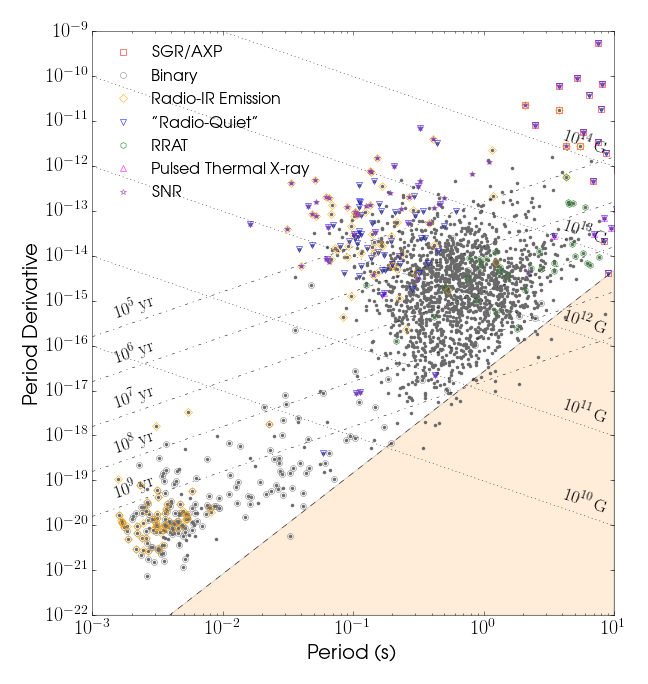
\includegraphics{ppdot.png}
\caption{A plot of pulsar period vs.~period derivative as produced using
\emph{psrqpy}}
\end{figure}

If requested the module can also return references for parameter values
for pulsars using the \texttt{ads} Python module (Sudilovsky et al.
2017).

Development of \emph{psrqpy} happens on Github (Pitkin 2017) and the
documentation is provided \href{http://psrqpy.readthedocs.io}{here}.

\hypertarget{refs}{}
\leavevmode\hypertarget{ref-matplotlib}{}%
Hunter, John D. 2007. ``Matplotlib: A 2D Graphics Environment.''
\emph{Computing in Science and Engineering} 9 (3): 90--95.
\url{https://doi.org/10.1109/MCSE.2007.55}.

\leavevmode\hypertarget{ref-ATNF}{}%
Manchester, R. N., G. B. Hobbs, A. Teoh, and M. Hobbs. 2005. ``The
Australia Telescope National Facility Pulsar Catalogue.''
\emph{Astronomical Journal} 129 (April): 1993--2006.
\url{https://doi.org/10.1086/428488}.

\leavevmode\hypertarget{ref-psrqpy_github}{}%
Pitkin, Matthew. 2017. ``Psrqpy on Github.'' 2017.
\url{https://github.com/mattpitkin/psrqpy}.

\leavevmode\hypertarget{ref-ADS}{}%
Sudilovsky, V., A. Casey, G. Barentsen, D. Foreman-Mackey, de Val-Borro.
M., and J. Elliott. 2017. ``The Ads Python Package.'' 2017.
\url{https://ads.readthedocs.io/}.

\end{document}
